% Contributions are much appreciated, in order to contribute to this project, head over to this repository:
% https://github.com/bshramin/uofa-eng-assignment

\documentclass[11pt,letterpaper]{article}
\textwidth 6.5in
\textheight 9.in
\oddsidemargin 0in
\headheight 0in
\usepackage{graphicx}
\usepackage{fancybox}
\usepackage[utf8]{inputenc}
\usepackage{epsfig,graphicx}
\usepackage{multicol,pst-plot}
\usepackage{pstricks}
\usepackage{amsmath}
\usepackage{amsfonts}
\usepackage{amssymb}
\usepackage{eucal}
\usepackage[left=2cm,right=2cm,top=2cm,bottom=2cm]{geometry}
\usepackage{esvect}
\pagestyle{empty}
\DeclareMathOperator{\tr}{Tr}
\newcommand*{\op}[1]{\check{\mathbf#1}}
\newcommand{\bra}[1]{\langle #1 |}
\newcommand{\ket}[1]{| #1 \rangle}
\newcommand{\braket}[2]{\langle #1 | #2 \rangle}
\newcommand{\mean}[1]{\langle #1 \rangle}
\newcommand{\opvec}[1]{\check{\vec #1}}
\renewcommand{\sp}[1]{$${\begin{split}#1\end{split}}$$}

\usepackage{lipsum}

\usepackage{listings}
\usepackage{color}
\usepackage{wrapfig}
\usepackage[shortlabels]{enumitem}

\definecolor{codegreen}{rgb}{0,0.6,0}
\definecolor{codegray}{rgb}{0.5,0.5,0.5}
\definecolor{codepurple}{rgb}{0.58,0,0.82}
\definecolor{backcolour}{rgb}{0.95,0.95,0.92}

\lstdefinestyle{mystyle}{
	backgroundcolor=\color{backcolour},   
	commentstyle=\color{codegreen},
	keywordstyle=\color{magenta},
	numberstyle=\tiny\color{codegray},
	stringstyle=\color{codepurple},
	basicstyle=\footnotesize,
	breakatwhitespace=false,         
	breaklines=true,                 
	captionpos=b,                    
	keepspaces=true,                 
	numbers=left,                    
	numbersep=5pt,                  
	showspaces=false,                
	showstringspaces=false,
	showtabs=false,                  
	tabsize=2
}

\lstset{style=mystyle}

\begin{document}
\pagestyle{plain}

\begin{flushleft}
Estudiante: Fabio Quimbay\\
Email: fabio.quimbay883@comunidadunir.net\\
Profesor: Miguel Ángel Cabeza\\
Fecha: Noviembre 14 de 2022\\
\end{flushleft}

\begin{flushright}\vspace{-20mm}

\includegraphics[height=2cm]{logo.png}
\end{flushright}
 
\begin{center}\vspace{0cm}
\textbf{\large PER5786 2022-2023  Física 1 (GFI) - PER5786 2022-2023}\\
 Tema 3 - Movimientos elementales
\end{center}

 
\rule{\linewidth}{0.1mm}
%%%%%%%%%%%%%%%%%%%%%%%%%%%%%%%%%%%%%%%%%%%%%%%%%%%%%%%%%%%%%%%%%%%%%%%%

\bigskip
\bigskip

%%%%%%%%%%%%%%%%%%%%
\textbf{Problema propuesto 9}\\

Un muelle con una masa oscila realizando un ciclo por segundo. Su recorrido total es de 10 cm. Inicia su movimiento desde un desplazamiento partiendo de uno de los extremos de su recorrido. Calcula su posición pasados 10 segundos.

\begin{wrapfigure}{r}{0.25\textwidth}
\begin{center}
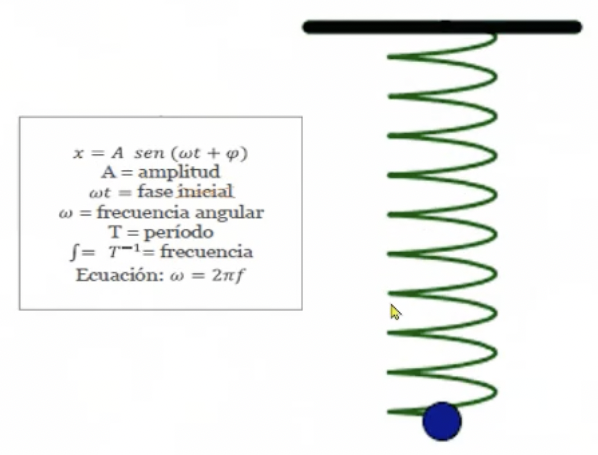
\includegraphics[width=0.25\textwidth]{problema_9.png}
\end{center}
\end{wrapfigure}

\textbf{Formulas base:}\\

Se tomarán las siguientes formulas base del MAS:

\begin{align}
\boxed{ X = A \cdot sin (\omega \cdot t + \varphi)} 
\end{align}

\textbf{Solución:}\\

Primero es necesario establecer todos los parámetros en términos de las unidades del SI, a saber:

\begin{align}
f &= 1\,ciclo/s = 1\,Hz\\ 
A &= 10\,cm = \frac{0.1}{2} = 0.05\,(al\,punto\,de\,origen)
\end{align}

Es importante tener presente que al comenzar en uno de sus extremos en necesario usar la función y/o desfase acorde, dado que la función seno comienza en 0, es necesario adicionarle un desfase de $\pi/2$ y si se usa la función no será necesario agregarle dicho desfase, dado que esta ya comienza en uno de los extremos, a saber:

\begin{align}
X_{t=10} = A \cdot sin (\omega \cdot t + \varphi) = 0.05 \cdot sin(2 \cdot \pi \cdot 10 + \frac{\pi}{2}) = 0.05\\
X_{t=10} = A \cdot sin (\omega \cdot t + \varphi) = 0.05 \cdot cos(2 \cdot \pi \cdot 10) = 0.05
\end{align}

De tal forma, la posición pasados 10 segundos, será de $0.05\,m$ equivalente a $5\,cm$.

%%%%%%%%%%%%%%%%%%%%

\end{document}

